

%% AP Physics MC Questions Archive
%%----------------------------------------


%% Static Friction
%%----------------------------------------
\element{ap}{
\begin{question}{static-friction-q01}
    Base your answer to the following question on the picture below which shows a \SI{3}{\kilo\gram} block sliding \SI{50}{\meter} down a frictionless inclined plane dropping a distance of \SI{30}{\meter}.
    \begin{center}
    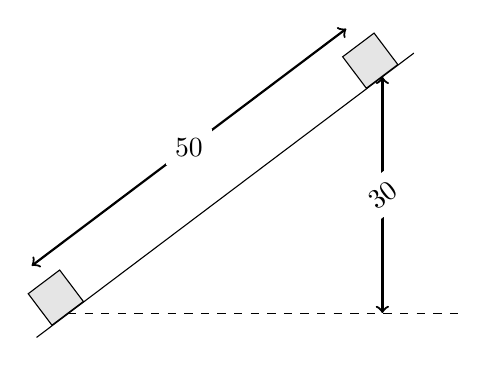
\begin{tikzpicture}
        %% Plane
        \draw (0,0) -- (37:6);
        %% Blocks
        \node[draw,rotate=37,anchor=south,minimum size=0.5cm,fill=white!90!black] (A) at (37:0.5) {};
        \node[draw,rotate=37,anchor=south,minimum size=0.5cm,fill=white!90!black] (B) at (37:5.5) {};
        %% Lables
        \draw[<->,thick] (A.north) ++(127:0.25) -- ++(37:5) node[pos=0.5,anchor=center,fill=white] {\SI{50}{\meter}};
        \draw[<->,thick] (37:5.5) --++(270:3) node[fill=white,pos=0.5,rotate=37.5,anchor=center] {\SI{30}{\meter}};
        \draw[dashed] (37:0.5) -- ++(0:5);
    \end{tikzpicture}
    \end{center}
    What is the minimum coefficient of static friction needed to prevent the block from moving?
    \begin{multicols}{3}
    \begin{choices}
        \wrongchoice{\num{1/3}}
        \wrongchoice{\num{3/5}}
      \correctchoice{\num{3/4}}
        \wrongchoice{\num{4/5}}
        \wrongchoice{\num{5/3}}
    \end{choices}
    \end{multicols}
\end{question}
}

\element{ap}{
\begin{question}{static-friction-q02}
    A \SI{3}{\kilo\gram} block is supported on a \ang{60} incline by a string as shown below.
    \begin{center}
    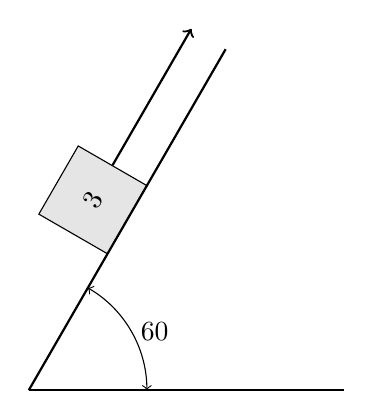
\begin{tikzpicture}
        %% incline
        \draw[thick] (0,0) -- ++(60:5);
        \draw[thick] (0,0) -- (4,0);
        \draw[<->] (1.5,0) arc (0:60:1.5) node[pos=0.5,anchor=west] {\ang{60}};
        %% block
        \node[draw,anchor=south,rotate=60,minimum size=1cm,fill=white!90!black] (A) at (60:2.5) {\SI{3}{\kilo\gram}};
        %% string
        \draw[thick,->] (A.east) -- ++(60:2);
    \end{tikzpicture}
    \end{center}
    If the coefficient of static friction is \num{1.0},
        the tension in the string is most nearly:
    \begin{multicols}{3}
    \begin{choices}
        \wrongchoice{\SI{5.3}{\newton}}
      \correctchoice{\SI{10.8}{\newton}}
        \wrongchoice{\SI{15}{\newton}}
        \wrongchoice{\SI{25.5}{\newton}}
        \wrongchoice{\SI{30}{\newton}}
    \end{choices}
    \end{multicols}
\end{question}
}

\element{ap}{
\begin{question}{static-friction-q03}
    A \SI{20}{\kilo\gram} block is held at rest on a ramp that makes an angle of \ang{30} with the horizontal.
    The coefficient of static friction between the block and the ramp is 0.7 and the coefficient of kinetic friction is 0.6.
    If the block is released, it will:
    \begin{choices}
      \correctchoice{remain stationary}
        \wrongchoice{begin to accelerate down the ramp, then decelerate and stop}
        \wrongchoice{accelerate down the ramp}
        \wrongchoice{move down the ramp with constant velocity}
        \wrongchoice{accelerate down the ramp until it reaches a terminal velocity,
            then remain traveling at that constant velocity}
    \end{choices}
\end{question}
}

\element{ap}{
\begin{question}{static-friction-q04}
    A \SI{50}{\kilo\gram} mass is placed on a inclined plane that makes an angle of \ang{37} with the horizontal.
    When released, the mass remains motionless.
    The coefficient of static friction between the mass and the plane is at least:
    \begin{multicols}{3}
    \begin{choices}
        \wrongchoice{0.1}
        \wrongchoice{0.2}
        \wrongchoice{0.4}
        \wrongchoice{0.5}
      \correctchoice{0.8}
    \end{choices}
    \end{multicols}
\end{question}
}

\element{ap}{
\begin{question}{static-friction-q05}
    A box weighing \SI{100}{\newton} is at rest on a horizontal surface.
    The coefficient of static friction between the box and the surface is 0.5,
        and the coefficient of kinetic friction is 0.25.
    If the crate is pushed with a force of \SI{20}{\newton} parallel to the floor,
        which of the following is true?
    \begin{choices}
        \wrongchoice{The crate will remain stationary, due to the static friction force of \SI{50}{\newton} which opposes the intended motion.}
      \correctchoice{The crate will remain stationary, due to the static friction force of \SI{20}{\newton} which opposes the intended motion.}
        \wrongchoice{The crate will accelerate across the floor at \SI{3}{\meter\per\second\squared}.}
        \wrongchoice{The crate will accelerate at until it reaches \SI{3}{\meter\per\second} then remain traveling at that constant velocity.}
        \wrongchoice{The crate will accelerate at \SI{3}{\meter\per\second\squared}, then its acceleration will increase to \SI{5}{\meter\per\second\squared}.}
    \end{choices}
\end{question}
}

\element{ap}{
\begin{question}{static-friction-q06}
    Block $A$ with mass $m$ is placed on a horizontal surface.
    The static coefficient of friction between $A$ and the surface is 0.6.
    The magnitude of the force necessary to push it across the surface at a constant velocity is $F_1$.
    Block $B$, also of mass $m$ is placed on top of the first block.
    The static coefficient of friction between $A$ and $B$ is 0.5.
    The force necessary to push this stack across the floor at constant velocity,
        $F_2$, is greater than $F_1$ because:
    \begin{choices}
        \wrongchoice{the force of friction on Block $B$ is greater}
        \wrongchoice{the coefficient of friction between Block $A$ and the floor is greater}
        \wrongchoice{the weight of Block $A$ is greater}
      \correctchoice{the force of the floor on Block $A$ is greater}
        \wrongchoice{of the additional frictional force between Block $A$ and Block $B$}
    \end{choices}
\end{question}
}

\element{ap}{
\begin{question}{static-friction-q07}
    Two boxes, each weighing \SI{900}{\newton} are stacked on a horizontal floor.
    Box $A$ is on the bottom,
        Box $B$ is on the top.
    The coefficient of static friction between Box $A$ and the floor is 0.3.
    A worker applies a force of \SI{600}{\newton} to Box $B$ parallel to the floor,
        and the stack moves together along the floor.
    Which of the following could be the coefficient of static friction between Box $A$ and Box $B$?
    \begin{multicols}{3}
    \begin{choices}
      \correctchoice{0.7}
        \wrongchoice{0.5}
        \wrongchoice{0.4}
        \wrongchoice{0.3}
        \wrongchoice{0.1}
    \end{choices}
    \end{multicols}
\end{question}
}

\element{ap}{
\begin{question}{static-friction-q08}
    Two crates are stacked on top of each other on a horizontal floor.
    The coefficient of static friction between Box $A$ and Box $B$ is 0.6.
    The coefficient of static friction between Box $A$ and the floor is 0.2.
    A force of \SI{100}{\newton} is applied parallel to the floor on Box $B$.
    The boxes move together along the floor.
    The ratio of the mass of Box $A$ to Box $B$ is possibly:
    \begin{multicols}{3}
    \begin{choices}
        \wrongchoice{$5:1$}
        \wrongchoice{$5:2$}
        \wrongchoice{$4:1$}
        \wrongchoice{$3:1$}
      \correctchoice{$1:2$}
    \end{choices}
    \end{multicols}
\end{question}
}

\element{ap}{
\begin{question}{static-friction-q09}
    An object of mass $m$ is placed on an inclined plane that makes an angle of $\theta$ with the horizontal.
    When released, the object remains stationary.
    The coefficient of static friction between the object and the plane is $\mu$.
    Which of the following must be true?
    \begin{multicols}{2}
    \begin{choices}
      \correctchoice{$\mu\cos\theta\geq\sin\theta$}
        \wrongchoice{$\mu\sin\theta\geq\cos\theta$}
        \wrongchoice{$\mu\sin\theta = \dfrac{1}{2}\cos\theta$}
        \wrongchoice{$\mu\cos\theta < \sin\theta$}
        \wrongchoice{$\mu\cos\theta\leq\sin\theta$}
    \end{choices}
    \end{multicols}
\end{question}
}

\element{ap}{
\begin{question}{static-friction-q10}
    What is the work done by friction on an \SI{10}{\newton} object that is initially at rest on a surface with a coefficient of static friction of 0.8 when the object is pushed by a \SI{7}{\newton} force for \SI{10}{\second}?
    \begin{multicols}{2}
    \begin{choices}
      \correctchoice{\SI{0}{\joule}}
        \wrongchoice{\SI{10}{\joule}}
        \wrongchoice{\SI{20}{\joule}}
        \wrongchoice{\SI{70}{\joule}}
        \wrongchoice{\SI{80}{\joule}}
    \end{choices}
    \end{multicols}
\end{question}
}

\element{ap}{
\begin{question}{static-friction-q10}
    Compared to the force of friction felt by an object which has a force exerted on it sliding on a rough surface,
        the force of friction felt by the object which has an equal force exerted on it while remaining at rest on the same surface:
    \begin{choices}
        \wrongchoice{is the same}
      \correctchoice{is greater}
        \wrongchoice{is lesser}
        \wrongchoice{depends on the nature of the object and the surface}
        \wrongchoice{virtually zero}
    \end{choices}
\end{question}
}


\endinput


